\chapter{Cascade de Transducteurs}
\label{chap-cassys}

Ce chapitre présente l'outil \textit{CasSys} qui donne la possibilité de créer une cascade
de  transducteurs et de nouvelles manières de travailler sur la langue naturelle avec des 
graphes à états finis. Une \textit{cascade de transducteurs} \index{cascade de transducteurs}
applique plusieurs graphes (automates ou transducteurs), l'un après l'autre, sur le texte: chaque
graphe modifie le texte, et les changements peuvent être utilisés pour des traitements supplémentaires
par les graphes suivants. Ce type de  système est notamment utilisé pour l'analyse syntaxique, le parenthésage (chunking),
l'extraction d'information, la reconnaissance d'entités nommées, etc. Pour faire cela, CasSys utilise
une succession de "locate pattern" avec les options adéquates.

\bigskip
\noindent Le premier prototype du système \textit{CasSys} \index{CasSys}  a été créé en 2002 au 
laboratoire LI (Laboratoire d'informatique de l'université de Tours) (\cite{these-nathalie}). 
Ce prototype était entièrement spécialisé pour l'extraction d'entités nommées. CasSys a été  
ensuite généralisé pour effectuer n'importe quelle sorte de traitement nécessitant une cascade. 
Il a été constamment amélioré au cours des années, puis intégré à Unitex, dans le cadre d'un projet\footnote{"Feder-Région Centre entités nommées et nommables" 
dirigé par Denis Maurel, LI, Tours, France, intégration réalisée par Nathalie Friburger et
David Nott}.

\bigskip
\noindent Les grammaires Unitex sont de type Context free et intègrent la notion de transduction issue
du domaine des automates à états finis. Une grammaire avec transduction (un  transducteur) est
capable de produire une sortie. CasSys est spécialisé dans l'application de transducteurs sous
la forme d'une cascade.

\bigskip
\noindent
Les transducteurs sont intéressants car ils permettent d'associer à la séquence
reconnue l'information qui se trouve dans les sorties des graphes.
Ces  sorties peuvent:
\begin{itemize}
\item Être ajoutées à la séquence reconnue et apparaître dans la concordance résultante ou le texte modifié.
\item Remplacer la séquence reconnue pour modifier le texte.
\end{itemize}
\noindent Ces deux  opérations transforment le texte ou lui ajoute des informations.

\bigskip
\noindent Dans ce chapitre, nous expliquons comment créer des cascades de transducteurs et
comment les appliquer. Ensuite, nous détaillons les options et possibilités offertes par CasSys.

%%%%%%%%%%%%%%%%%%%%%%%%%%%%%%%%%%%%%%%%%%%%%%%%%%%%%%%%%%%%%
\section{Appliquer une cascade de Transducteurs avec CasSys}
\label{section:applyCascade}
Appliquer une cascade de transducteurs avec CasSys consiste à représenter un phénomène linguistique par une
liste de transducteurs à appliquer au texte dans un ordre précis: CasSys et son interface dans Unitex permettent d'y parvenir.
Cette section explique comment utiliser l'interface pour créer et gérer les graphes (ordre, ajout, suppression) et appliquer la cascade.   

%%%%%%%%%%%%
\subsection{Création de la liste des transducteurs}
\label{subsec:listTrans}

\bigskip
\noindent Afin de pouvoir gérer la liste de transducteurs, le menu FSGraph comporte deux sous-menus:
"\textit{New cascade}" et "\textit{Edit cascade...}" (Figure~\ref{fig13-08}). Pour créer la liste des
transducteurs, sélectionnez "\textit{New cascade}". Si vous souhaitez modifier une cascade existante, sélectionnez
"\textit{Edit cascade...}", puis  choisissez le nom de la cascade à ouvrir.

\begin{figure}[!htb]
 \centering
 \includegraphics[width=4cm]{resources/img/fig13-08.png}
 \caption{Menu "FSGraph" d'Unitex et sous-menu "New Cascade" et "\textit{Edit cascade...}"}
 \label{fig13-08}
\end{figure}

Le répertoire de la langue courante contient un sous-répertoire nommé CasSys dans lequel se trouvent
les fichiers de configuration d'une cascade. Ce sont des fichiers textes avec l'extension \textit{.csc} (ex: maCascade.csc)

\subsection{\'{E}dition de la liste des transducteurs}
\label{subsec:editlistTrans}

La fenêtre de configuration de CasSys (Figure~\ref{fig13-03}) comporte trois parties :

\begin{figure}[!htb]
  \centering
  \includegraphics[width=16cm]{resources/img/fig13-03.png}
  \caption{Fenêtre de configuration de CasSys avec à droite la liste des transducteurs}
  \label{fig13-03}
\end{figure}

\begin{enumerate}
	\item Un \textit{gestionnaire de fichier} à gauche du cadre permet de choisir les transducteurs à mettre dans la cascade.
	Le gestionnaire n'affiche que les fichiers \emph{fst2} (tous les graphes que vous souhaitez mettre dans la liste doivent être compilés au format \textit{fst2}).
	
	Pour éditer la cascade, choisissez les graphes à gauche et mettez-les à droite à l'aide d'un glisser-déposer.
\item Le \textit{tableau} de droite affiche la cascade: la liste ordonnée des transducteurs et les options sélectionnées pour chaque graphe.
		Le tableau est évidemment vide pour une nouvelle cascade.
		 
		Les colonnes du tableau (Figure~\ref{fig13-09}) donne le numéro de chaque graphe et permettent de choisir leur comportement.
	\begin{itemize}
	\item \textbf{\#} : Numéro du graphe/transducteur dans la cascade pour chaque graphe; le fichier \emph{fst2} est numéroté.
	\item \textbf{Disabled} : Pour désélectionner le graphe courant. \textit{Disabled} siginifie: "\textit{non appliqué dans la cascade}".
		Les graphes non sélectionnés apparaissent sans numéro, en grisé et barré.
	\item \textbf{Name} : Le nom du graphe (avec l'extension \emph{fst2}). Si vous laissez la souris sur le nom du graphe,
		une info-bulle apparaît avec le chemin complet du graphe (depuis le répertoire courant \emph{Graphs}).
		Les graphes dont le fichier source n'est pas trouvé apparaissent en italique et en rouge.

	\item \textbf{Merge}: Si le transducteur doit être appliqué en mode \textit{merge}.
	\item \textbf{Replace}: Si le transducteur doit être appliqué en mode \textit{replace}.
	\item \textbf{Until fix point}: Si le transducteur doit être appliqué une ou plusieurs fois
		jusqu'à ce que le texte reste inchangé, c'est-à-dire jusqu'à ce qu'un point fixe soit atteint (voir \ref{sub:AppWhiCon}).
	\end{itemize}
	
	 \item Au centre se trouvent les boutons décrits ci-dessous:
		\begin{itemize}
		\item \textit{"Up"/"Down"/"Top"/"Bottom"} sont utilisés pour modifier l'ordre
		des transducteurs dans la liste (ils déplacent le transducteur sélectionné); 
		\textit{"Up"} et \textit{"Down"} déplacent le transducteur sélectionné d'une ligne vers le haut ou
			vers le bas, \textit{"Top"} et \textit{"Bottom"} le positonnent au début ou à la fin de la liste.
		\item \textit{"Delete"} permet de supprimer le transducteur sélectionné de
		la liste des transducteurs. 
		\item \textit{"Add"} ajoute un transducteur (précédemment sélectionné) dans la liste.
			Il remplace le gisser-déposer préalablement décrit.
		\item \textit{"View"} ouvre le graphe sélectionné aussi bien dans l'explorateur
		de fichiers que dans la liste de transducteurs. Il est très utile d'avoir un accès
		rapide à n'importe quel transducteur aussi bien pour y jeter un coup d'œil que pour
		le modifier.
		\item \textit{"Save"} et \textit{"Save as"} permettent d'enregistrer la
		liste des transducteurs. Par défaut, les listes des transducteurs sont placées dans
		le répertoire CasSys de la langue courante  (par exemple French/CasSys).
		\item \textit{"Compile"} recompile tous les graphes de la cascade.	
		\item \textit{"Disable all"} pour désélectionner tous les graphes de la cascade.	
		\item \textit{"Enable all"} pour sélectionner tous les graphes de la cascade.	
		\item \textit{"Close"} ferme la fenêtre courante.
		\end{itemize}
\end{enumerate}


\begin{figure}[!htb]
  \centering
  \includegraphics[width=7cm]{resources/img/fig13-09.png}
  \caption{La table/liste de transducteurs}
  \label{fig13-09}
\end{figure}

	

\subsection{Application d'une cascade}
\label{subsec:launchCascade}

Dans le menu "Text", sélectionner le sous-menu "\textit{Apply CasSys cascade...}" (Figure~\ref{fig13-01}) pour ouvrir la fenêtre CasSys.
Ce sous-menu "\textit{Apply CasSys cascade...}" n'est actif que si un texte a été préalablement ouvert.

\begin{figure}[!htb]
 \centering
 \includegraphics[width=5cm]{resources/img/fig13-01.png}
 \caption{Menu "Text" d'Unitex et sous-menu "Apply CasSys Cascade"}
 \label{fig13-01}
\end{figure}

La fenêtre CasSys (Figure~\ref{fig13-02}) affiche le contenu du répertoire CasSys de la langue courante. Elle
permet de choisir le fichier contenant la liste de transducteurs à appliquer au texte. Une fois que cette liste
est choisie, vous pouvez cliquer sur le bouton "Launch" pour appliquer la cascade. Attention, pour que l'affichage se fasse ici, il faut obligatoirement que le nom du fichier contenant la liste de transducteurs ait pour extension \verb+.csc+.

\begin{figure}[!htb]
  \centering
  \includegraphics[width=10cm]{resources/img/fig13-02.png}
  \caption{Fenêtre de lancement de la cascade de transducteurs}
  \label{fig13-02}
\end{figure}

N'importe quel dictionnaire du mode morphologique déclaré dans vos préférences est utlisable dans vos
graphes.
Les  préférences peuvent être modifiées à partir du menu "Info" (Info -->
Preferences --> morphological-mode dictionaries).

%%%%%%%%%%%%%%%%%%%%%%%%%%%%%%%%%%%%%%%%%%%%%%%%%%%%%%%
\section{CasSys en détail}

Dans cette section nous présentons une description détaillée du fonctionnement de CasSys.

\subsection{Type de graphe utilisé}
\label{graphs-for-cassys}

CasSys utilise la version compilée des graphes (format \verb+.fst2+). CasSys gère les grammaires locales
(section~\ref{syntactic-graphs}) présentées dans le chapitre \ref{chap-advanced-grammars}.
Les grammaires utilisées dans une cascade suivent les mêmes règles que les grammaires habituellement
utilisées dans Unitex. Elles peuvent comporter des sous-graphes, utiliser le mode morphologique et les filtres
morphologiques, et faire référence aux informations présentes dans les dictionnaires. 

\bigskip
\noindent CasSys n'est pas compatible avec les fichiers \verb+fst2+ en mode debug (section~\ref{section-debug-mode}).
Quand on applique un graphe en mode debug avec le menu \verb+Text>Locate Pattern+, le système
compile le graphe dans un format spécial de mode debug. Pour obtenir un fichier au format \verb+fst2+ normal,
recompilez le graphe, soit avec le menu \verb+FSGraph+, soit en ligne de commande, soit en décochant le mode
debug avant d'appliquer le graphe avec \verb+Locate Pattern+.

\subsection{Application itérative}
\label{sub:AppWhiCon}

CasSys peut appliquer un graphe sur un texte de manière itérative tant que de nouvelles concordances sont obtenues.
Ce comportement est sélectionné ou non pour chaque graphe selon que la case \verb+Until fix point+ est cochée ou non. Cette section présente le comportement de cette option\\

Considérons par exemple le graphe \ref{fig:AB->A} qui reconnait \emph{AB} et le remplace par \emph{A}.\\

\begin{figure}[!htbp]
  \centering
  \includegraphics[width=6cm]{resources/img/AB_to_A.png}
  \caption{Transducteur qui modifie BA en A}
  \label{fig:AB->A}
\end{figure}

Considérons le texte \emph{B B B A A A}. L'application du graphe \ref{fig:AB->A} sur ce texte avec \emph{Until fix point}  donne :\\

\begin{tabular}{|l|cccccc|r|}
\hline
initial text  &B&B&B&A&A&A&\\
\hline
itération 1 & &B&B&A&A&A& 1 match\\
itération 2 & & &B&A&A&A& 1 match\\
itération 3 & & & &A&A&A& 1 match\\
itération 4 & & & &A&A&A& 0 match\\
\hline
\end{tabular}

\bigskip
Durant les trois premières itérations, une concordance est obtenue, le graphe
est alors appliqué à nouveau au texte résultant. A la quatrième itération, aucune
concordance n'est trouvée, le graphe n'est donc plus réappliqué.

\bigskip
\large{\textbf{Attention :}} Prendre garde à la possibilité de blocage en utilisant cette 
option. Par exemple, un transducteur qui reconnaît \emph{A} et le remplace par
\emph{A} causerait un blocage s'il était appliqué sur le texte de l'exemple.

\begin{comment}
\subsection{Un texte au format de type XML avec étiquettes lexicales}

En sortie, le format avec étiquettes lexicales est transformé en un format de type XML.
Ce changement est fait dans le but de proposer un texte plus manipulable  à l'utilisateur final.

A partir de ce format, il est plus facile d'obtenir une sortie adaptable à tous.\\

Plus précisément, les étiquettes lexicales :\\
\begin{tabular}{c}
\texttt{
\{forme.lemme,code1+code2:flex1:flex2\}}
\end{tabular}\\

La sortie CaSsys de type XML a le format suivant :\\
\begin{tabular}{ll}
\texttt{<csc>}&\\
	&\texttt{<form>forme</form>}\\
	&\texttt{<lem>lemme</lem>}\\
	&\texttt{<code>code1</code>}\\
	&\texttt{<code>code2</code>}\\
	&\texttt{<inflect>flex1</inflect>}\\
	&\texttt{<inflect>flex2</inflect>}\\
\texttt{</csc>}&\\
\end{tabular}
\end{comment}


\subsection{Règles utilisées dans une cascade}

Dans une cascade, chaque graphe observe les règles utilisées dans Unitex:
\begin{itemize}
	\item Insertion à gauche des motifs reconnus : en mode "merge", la sortie est insérée à
	gauche de la séquence reconnue.
	\item	Priorité au motif le plus à gauche : lors de l'application d'une grammaire locale,
	les occurrences qui se chevauchent sont toutes indexées. 
	Durant la construction de la concordance, toutes ces occurrences sont présentes, mais comme CasSys
	modifie le texte après application de chaque 
	graphe de la cascade, il est nécessaire de choisir parmi ces occurrences celle à prendre en
	compte. La priorité est donnée à la séquence la plus à gauche.
	\item Priorité au plus long motif: dans CasSys, lors de l'application d'un graphe, c'est la
	séquence la plus longue qui est conservée.
	\item	Limitation du nombre d'occurrences recherchées: dans CasSys, ce nombre n'est pas
	limité : une telle limitation n'a aucun sens dans CasSys. Toutes les occurrences sont
	toujours indexées dans le texte.
\end{itemize}

\subsection{Marquage de motifs dans CasSys}

La sortie des transducteurs peut être utilisée pour insérer des informations dans les textes, en
particulier pour marquer les motifs reconnus: il est possible d'utiliser toute sorte de marques, 
( ), [], "", etc. ou des balises xml comme <xxx> </xxx>, mais CasSys propose une manière
particulière d'annoter les motifs reconnus, offrant certaines possibilités que nous présentons
maintenant.  

\bigskip
\noindent Unitex découpe les textes en tokens de différentes sortes comme le marqueur de fin de
phrase \{S\}; le marqueur {STOP}, des séquences de lettres contiguës, des étiquettes lexicales
{aujourd'hui,.ADV}, etc. Les étiquettes lexicales sont utilisées dans CasSys de manière
particulière. Une étiquette lexicale (entre accolades) est habituellement utilisée pour éviter les
ambiguïtés (voir les explications à la section \ref{tokenization} et à la section
\ref{section-displaying-sentence-automata}). 
Par exemple, dans un texte, si vous avez le token \emph{\{curly brackets,.N\}}, ni "curly" ni
"brackets" ne seront reconnus, mais seulement la séquence toute entière
"curly brackets". Une étiquette lexicale peut contenir une information lexicale complexe comme
\emph{N+Pers+Hum:fs}.
Dans un graphe, il est possible de chercher un token en utilisant l'information contenue dans un
masque lexical : par exemple, on peut écrire \emph{<.N>} pour chercher 
un nom, \emph{<.Pers+Hum>} pour un être humain ou \emph{<.Pers>}. Ces masques lexicaux sont décrits
dans le chapitre "Recherche d'expressions rationnelles" section
\ref{section-special-symbols}.
 
\bigskip
\noindent Dans CasSys, nous utilisons la marque lexicale de manière particulière. Une cascade de
transducteurs est intéressante pour localiser un îlot de certitude. Il est nécessaire pour ce type
de système d'éviter que des motifs précédemment reconnus soient ambigus avec ceux reconnus par les
graphes suivants. Pour éviter cela, on étiquette les motifs reconnus par les graphes sous la forme
\emph{\{} et \emph{,.tag1+tag2+tagn\}} (où \emph{tag1, tag2, etc.} sont vos propres étiquettes).

\bigskip
\noindent Pour expliciter ce comportement, voici un exemple très simple. Le texte sur lequel nous
travaillons est :

\emph{bac a b c cc a b b ba ab a b bca a b c abaabc}.

\bigskip
\noindent Le graphe grfAB (Figure~\ref{fig13-05}) reconnaît la séquence \emph{ab} dans le texte et lui
ajoute l'étiquette lexicale \{a b,.AB\}. Ce graphe appliqué en mode MERGE ajoute \emph{\{ } et
 \emph{,.AB\}} dans le texte.

\begin{figure}[!htb]
  \centering
  \includegraphics[width=6cm]{resources/img/fig13-05.png}
  \caption{Le graphe grfAB}
  \label{fig13-05}
\end{figure}

\bigskip
\noindent Le texte résultant est : \emph{bac \{a b,.AB\} c cc \{a b,.AB\} b ba ab \{a b,.AB\} bca
\{a b,.AB\} c abaabc}.

\bigskip
\noindent Maintenant le motif \emph{a b} est étiqueté \emph{AB}. La partie (a ou b seul) de ce
motif ne peut pas l'être à cause de l'étiquetage de \emph{a b}.

\bigskip
\noindent Après ce graphe, la cascade applique un autre graphe nommé "tagAB" (Figure~\ref{fig13-06})
contenant le masque lexical <AB>. Il reconnait toutes les séquences lexicalement étiquetées par le
graphe précédent.

\begin{figure}[!htb]
  \centering
  \includegraphics[width=10cm]{resources/img/fig13-06.png}
  \caption{Le graphe tagAB}
  \label{fig13-06}
\end{figure}

\bigskip
\noindent Le texte résultant est : \emph{bac \{\{a b,.AB\} c,.ABC\} cc \{a b,.AB\} b ba ab \{a
b,.AB\} \{bca,.BCA\} \{\{a b,.AB\} c,.ABC\} abaabc}.


\bigskip
\noindent La concordance affichée par Unitex devrait ressembler à celle de la figure~\ref{fig13-07}. Pour des raisons liées à la programmation (les ambiguïtés entre les
	caractères entre accolades des étiquettes lexicales), nous n'avons d'autres options que de
placer des  $\backslash$ avant chaque caractère ambigu; c'est pourquoi ces symboles sont précédés de
$\backslash$ dans la concordance pour éviter des problèmes avec Unitex.

\begin{figure}[!htb]
  \centering
  \includegraphics[width=15cm]{resources/img/fig13-07.png}
  \caption{La concordance issue l'application de la cascade}
  \label{fig13-07}
\end{figure}

\section{Graphes de g\'{e}n\'{e}ralisation d'\'{e}tiquetage}
\label{graph-generalization}

Parfois, on a identifi\'{e} des \'{e}l\'{e}ments recherch\'{e}s gr\^{a}ce \`{a} certains contextes,
mais si ces \'{e}l\'{e}ments apparaissent dans un autre contexte on ne les reconna\^{i}t pas.
Afin de trouver de telles occurrences, CasSys propose d'utiliser des graphes de
g\'{e}n\'{e}ralisation d'\'{e}tiquetage. Ces graphes contiennent des bo\^{i}tes vides
quer le programme remplit automatiquement avant d'appliquer les graphes
au texte. Les graphes de g\'{e}n\'{e}ralisation d'\'{e}tiquetage ne fonctionnent
qu'avec l'utilisation d'accolades, car le programme consulte la liste de tokens
(tokens.txt) du texte \`{a} analyser par le futur graphe.

\bigskip
\noindent Dans le cas d'un token comme:

\bigskip
\emph{\{\{mars,.mois\} \{2018,.année\},.date\}}

\bigskip
\noindent nous appellerons dans la suite \emph{sous-étiquettes lexicales} les éléments
\emph{\{mars,.mois\}} et \emph{\{2018,.année\}}, et \emph{sous-catégories}
les catégories \textit{mois} et \textit{année}.

\subsection{D\'{e}claration d'un graphe de g\'{e}n\'{e}ralisation d'\'{e}tiquetage}
Pour que CasSys reconnaisse un graphe de g\'{e}n\'{e}ralisation d'\'{e}tiquetage, il faut
cocher la colonne \emph{Generalization} (figure~\ref{fig12-3}).

\begin{figure}[!htb]
  \centering
  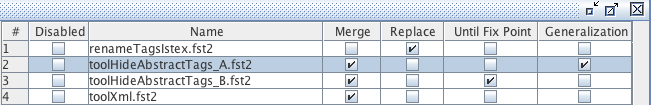
\includegraphics[width=15cm]{resources/img/fig12-3.png}
  \caption{Graphe de g\'{e}n\'{e}ralisation d'\'{e}tiquetage}
  \label{fig12-3}
\end{figure}

\subsection{Structure d'un graphe de g\'{e}n\'{e}ralisation d'\'{e}tiquetage}

\subsubsection{Graphe de généralisation d'étiquetage simple}

Pour créer un graphe de généralisation d'étiquetage, on marque le début de la partie
générique par une boîte \$G avec en sortie une accolade ouvrante, et la fin
par une boîte vide avec en sortie une accolade fermante éventuellement précédée
d'un ou plusieurs traits. Il faut placer entre les deux une (et une seule) boîte vide
avec en sortie l'élément à rechercher, précédé de ",.". Il est possible d'utiliser
le bouton \$G (figure~\ref{fig:bouton_g}) pour insérer automatiquement les boîtes
de début et de fin de la partie générique après avoir sélectionné une boîte.

\begin{figure}[!htb]
  \centering
  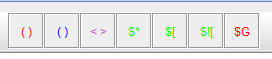
\includegraphics[width=8cm]{resources/img/bouton_g.png}
  \caption{Bouton \$G}
  \label{fig:bouton_g}
\end{figure}

\bigskip
\noindent Par exemple, si le fichier de tokens contient l'étiquette lexicale
\emph{\{A,.x\}}, le graphe générique de la figure~\ref{fig:graphe_generique_simple}
est conçu pour extraire les éléments de catégorie \textit{x} et son traitement va générer
le graphe en figure~\ref{fig:graphe_generique_simple_genere}. Un contexte droit négatif
est ajouté automatiquement pour empêcher un deuxième étiquetage des occurrences
déjà étiquetées. Attention cependant que les éléments de la boite sont des masques
lexicaux (voir la justification en section~\ref{tokenization}), ce qui peut créer une ambiguïté
avec un code grammatical. Le graphe de la figure~\ref{fig:graphe_generique_simple_genere}
est catastrophique de ce point de vue, car il reconnait tous les adjectifs du texte!

\begin{figure}[!htb]
  \centering
  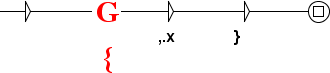
\includegraphics[width=8cm]{resources/img/graphe_generique_simple.png}
  \caption{Graphe de généralisation d'étiquetage simple}
  \label{fig:graphe_generique_simple}
\end{figure}

\begin{figure}[!htb]
  \centering
  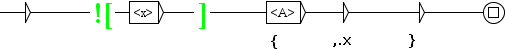
\includegraphics[width=10cm]{resources/img/graphe_generique_simple_genere.png}
  \caption{Graphe de généralisation d'étiquetage simple après traitement}
  \label{fig:graphe_generique_simple_genere}
\end{figure}

\bigskip
\noindent Remarque: lors de la création d'un graphe de généralisation d'étiquetage, plusieurs
parties génériques peuvent être insérées dans le graphe, et des boîtes classiques
peuvent être ajoutées avant et après chaque partie générique, comme le montre
la figure~\ref{fig:graphe_generique_plusieurs_chemins}.

\begin{figure}[!htb]
  \centering
  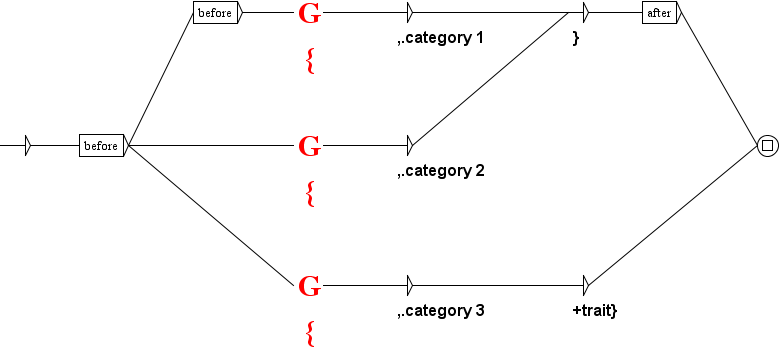
\includegraphics[width=14cm]{resources/img/graphe_generique_plusieurs_chemins.png}
  \caption{Graphe de généralisation d'étiquetage avec plusieurs chemins}
  \label{fig:graphe_generique_plusieurs_chemins}
\end{figure}

\subsubsection{Graphe de généralisation d'étiquetage avec restriction\protect\footnote{Dans
certaines versions 3.2 alpha, des restrictions négatives étaient présentes. Elles ne le sont plus,
mais le comportement d'une partie générique utilisant des restrictions négatives
peut être reproduit en utilisant des restrictions positives. Pour plus d'information ou
en cas de besoin, contacter la liste Google Unitex.}}

Les graphes simples permettent de récupérer le contenu des tokens de catégorie cherchée
du fichier tokens.txt, mais il peut arriver que l'on veuille récupérer le contenu d'une
sous-étiquette lexicale. Pour cela on peut utiliser des restrictions dans les graphes
de généralisation d'étiquetage. On place alors la sous-catégorie à rechercher
dans la boîte, tout en laissant en sortie la catégorie principale précédée de ",.".
Cette sous-catégorie doit être seule dans la boîte. Si on veut extraire plusieurs sous-catégories,
il faut créer plusieurs chemins.

\bigskip
Prenons un exemple, supposons que la ligne suivante soit présente dans le fichier tokens.txt:

\bigskip
\emph{\{\{first,.A\} \{\{second,.A\} \{third,.B\},.B\},.main\}}

\bigskip
\noindent et que l'on veuille extraire la sous-étiquette lexicale de sous-catégorie \textit{A}
ou celle de sous-catégorie \textit{B}.

\bigskip
\noindent Le graphe de la figure~\ref{fig:graphe_restriction_A} une fois traité donnera
le graphe en figure~\ref{fig:graphe_restriction_A_genere}, alors que le graphe en
figure~\ref{fig:graphe_restriction_B} donnera le graphe en
figure~\ref{fig:graphe_restriction_B_genere}.

\begin{figure}[!htb]
  \centering
  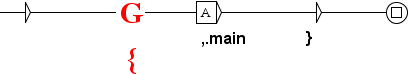
\includegraphics[width=8cm]{resources/img/graphe_restriction_A.png}
  \caption{Graphe de généralisation d'étiquetage avec une restriction sur la sous-catégorie A}
  \label{fig:graphe_restriction_A}
\end{figure}

\begin{figure}[!htb]
  \centering
  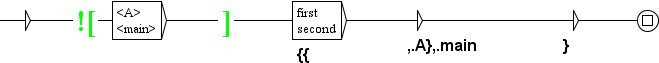
\includegraphics[width=14cm]{resources/img/graphe_restriction_A_genere.png}
  \caption{Graphe de généralisation d'étiquetage avec une restriction sur la sous-catégorie A
  après traitement}
  \label{fig:graphe_restriction_A_genere}
\end{figure}

\begin{figure}[!htb]
  \centering
  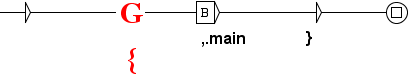
\includegraphics[width=8cm]{resources/img/graphe_restriction_B.png}
  \caption{Graphe de généralisation d'étiquetage avec une restriction sur la sous-catégorie B}
  \label{fig:graphe_restriction_B}
\end{figure}

\begin{figure}[!htb]
  \centering
  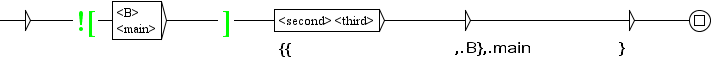
\includegraphics[width=14cm]{resources/img/graphe_restriction_B_genere.png}
  \caption{Graphe de généralisation d'étiquetage avec une restriction sur la sous-catégorie B
  après traitement}
  \label{fig:graphe_restriction_B_genere}
\end{figure}

\bigskip
\noindent Dans le premier cas, deux sous-étiquettes lexicales de sous-catégorie \textit{A}
ont été trouvées, "first" et "second". Dans le deuxième cas, une seule sous-étiquette
lexicale de sous-catégorie \textit{B} a été trouvée; cette sous-étiquette lexicale contient
elle-même deux autres sous-étiquettes lexicales; le contenu extrait est donc la concaténation
de ce qui se trouve à l'intérieur, c'est-à-dire "second third". Comme la sous-catégorie
correspondait, la recherche n'a pas été propagée aux sous-étiquettes lexicales
de niveau inférieur et la sous-étiquette lexicale "third" toute seule n'a pas été trouvée.

\bigskip
\noindent Par ailleurs, on remarque plusieurs choses: tout d'abord, le contexte droit négatif
contient maintenant la catégorie du token principal et la sous-catégorie recherchée; de plus,
les éléments trouvés sont doublement étiquetés, avec les deux catégories imbriquées.

\bigskip
\noindent Un graphe de généralisation d'étiquetage ne doit pas contenir un chemin
sans restriction et un chemin avec restriction pour la même catégorie, à cause de
l'ambiguïté qui en résulterait, sauf en utilisant des poids sur les chemins (voir
section~\ref{Transducers}), comme le montre la figure~\ref{fig:graphe_poids}.

\begin{figure}[!htb]
  \centering
  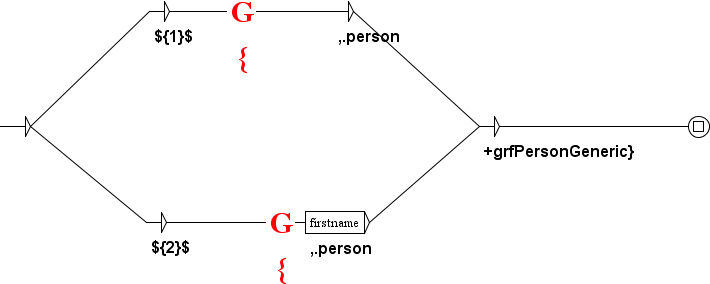
\includegraphics[width=10cm]{resources/img/graphe_poids.png}
  \caption{Graphe avec des poids pour éviter les ambiguïtés}
  \label{fig:graphe_poids}
\end{figure}

\subsubsection{Remplacement de la catégorie}

Dans certains cas, il peut arriver que l'on veuille modifier la catégorie qui sera indiquée
dans les sous-étiquettes lexicales que l'on extrait par un graphe de généralisation d'étiquetage.
Par exemple dans le cas suivant :

\bigskip
\noindent \emph{\{from \{\{january,.month\} \{2017,.year\},.date\} to \{\{novembre,.month\} \{2018,.year\},.date\},.period\}}


\bigskip
\noindent En utilisant un graphe de généralisation d'étiquetage avec restriction pour extraire
les années, les sous-étiquettes lexicales nouvellement trouvées seraient étiquetées
de la façon suivante:

\bigskip
\emph{\{\{2017,.year\},.period\}} et \emph{\{\{2018,.year\},.period\}}

\bigskip
\noindent Ici, on voudrait remplacer "period", qui ne représente pas très bien la catégorie
de ces sous-étiquettes lexicales, par "date".

\bigskip
\noindent Pour cela il est possible de préciser la catégorie finale à obtenir, en l'ajoutant
(après un point) à la sous-catégorie à rechercher (voir les figures~\ref{fig:graphe_remplacement}
et \ref{fig:graphe_remplacement_genere}).

\begin{figure}[!htb]
  \centering
  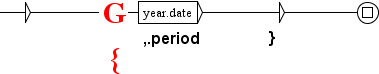
\includegraphics[width=10cm]{resources/img/graphe_remplacement.png}
  \caption{Graphe avec remplacement de la catégorie finale}
  \label{fig:graphe_remplacement}
\end{figure}

\begin{figure}[!htb]
  \centering
  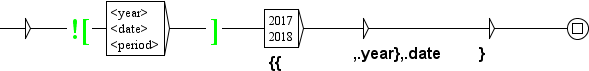
\includegraphics[width=10cm]{resources/img/graphe_remplacement_genere.png}
  \caption{Graphe avec remplacement de la catégorie finale après traitement}
  \label{fig:graphe_remplacement_genere}
\end{figure}

\section{Les résultats d'une cascade}

\subsection{Affichage des résultats de la cascade}
\label{subsec:resultsCascade}

Le résultat de l'application d'une cascade est un fichier d'index (\textit{concord.ind}), comme c'est le cas
lors d'une recherche de motif avec \textit{"Locate pattern"}. Ce fichier d'index contient toutes les séquences
reconnues conformément aux règles fixées dans Unitex.

\bigskip
\noindent Pour afficher une concordance, il suffit de cliquer sur le bouton "Build concordance"
(comme décrit au chapitre \ref{chap-advanced-grammars}) dans la menu "Text / Located sequences".
La figure~\ref{fig13-04} présente un échantillon de concordance d'une cascade qui reconnaît les entités
nommées.


\begin{figure}[!htb]
  \centering
  \includegraphics[width=14cm]{resources/img/fig13-04.png}
  \caption{Concordance de CasSys dans Unitex}
  \label{fig13-04}
\end{figure}

\subsection{Les différents fichiers résultats d'une cascade}

CasSys conserve tous les textes créés par chaque graphe  de la cascade. Ceci peut être
utile  pour des tests, le débogage ou la vérification de différents résultats de la cascade. Il est
alors possible de corriger les erreurs selon l'ordre d'application des graphes ou de trouver des
erreurs dans leur écriture. Il est pratique d'ajouter dans la sortie d'un transducteur le nom de ce
dernier, afin de voir dans le résultat final quel motif a été reconnu par quel graphe.

Si l'on applique une cascade au texte exemple.txt, deux répertoires sont créés:
\verb+exemple_snt+ et \verb+exemple_csc+.
Les fichiers créés dans \verb+exemple_csc+ sont les résultats obtenus par
chaque graphe. Ces fichiers sont intitulés selon le numéro du graphe qui les a produit. Par exemple, si le
troisième graphe reconnaît un motif, les résultats de l'application de ce graphe seront stockés dans le 
répertoire  \verb+exemple_3+\newline\verb+_0_snt+ le fichier \verb+exemple_3_0.snt+ contiendra le texte modifié.

\subsection{Un texte au format de type XML pour les étiquettes lexicales}

En sortie, le résultat est fourni sous deux formes~: le texte résultant directement de l'application
des transducteurs, et un format de type XML dans lequel les étiquettes lexicales ont été transformées en XML.
Ce changement est fait dans le but de proposer un texte plus manipulable  à l'utilisateur final.
A partir de ce format, il est possible d'utiliser l'un des nombreux outils de traitement du XML.
Il est également facile d'appliquer des transducteurs supplémentaires afin d'obtenir la sortie souhaitée.
Le texte résultant directement des transducteurs est sauvegardé dans le fichier  \verb+exemple_csc.raw+,
et la version  XML-isée est dans le fichier \verb+exemple_csc.txt+.

Plus précisement, les étiquettes lexicales sont dans le format suivant~:\\
\begin{tabular}{c}
\texttt{
\{forme.lemme,code1+code2:flex1:flex2\}}
\end{tabular}\\
La sortie de type XML correspondante a le format suivant~:\\
\begin{tabular}{ll}
\texttt{<csc>}&\\
	&\texttt{<form>forme</form>}\\
	&\texttt{<lemma>lemme</lemma>}\\
	&\texttt{<code>code1</code>}\\
	&\texttt{<code>code2</code>}\\
	&\texttt{<inflect>flex1</inflect>}\\
	&\texttt{<inflect>flex2</inflect>}\\
\texttt{</csc>}&\\
\end{tabular}

La DTD de notre format est la suivante~:

\begin{tabular}{l}
\texttt{<?xml version="1.0" encoding="ISO-8859-1"?>}\\
\texttt{<!ELEMENT text (\#PCDATA|csc)*>}\\
\texttt{<!ELEMENT csc (form,lemma?,code*,inflect*) >}\\
\texttt{<!ELEMENT form (\#PCDATA|csc)*>}\\
\texttt{<!ELEMENT lemma (\#PCDATA)>}\\
\texttt{<!ELEMENT code (\#PCDATA)>}\\
\texttt{<!ELEMENT inflect (\#PCDATA)>}\\
\end{tabular}

%%%%%%%%%%%%%%%%%%%%%%%%%%%%%%%%%%%%%%%%%%%%

\section{La création d'un inventaire d'occurrences balisées}
\label{section-standOff}

L'option \verb$standoff$ de CasSys (section~\ref{section-program-Cassys}) permet de traiter
un corpus balisé dans le style XML, et de produire un fichier résultat répertoriant les expressions du
corpus qui sont délimitées par des balises, avec le nombre d'occurrences de chaque expression distincte.
Cette option n'est pas disponible via l'interface d'Unitex et doit être lancée par un script
(chapitre~\ref{chap-scripts}) ou un programme externe.

\bigskip
\noindent Il faut fournir un graphe qui reconnait les éléments à rechercher (éléments au sens XML,
c'est-à-dire expressions délimitées par une balise ouvrante et la balise fermante correspondante).
Ce graphe aura généralement un contexte droit négatif (section~\ref{section-contexts}). 
Par exemple, le graphe de la figure~\ref{fig-placeNameStandoff} permet d'inventorier les expressions
balisées entre \verb$<placeName>$ et  \verb$</placeName>$.

\begin{figure}[!htb]
  \centering
  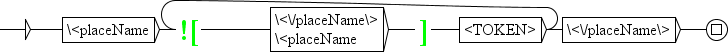
\includegraphics[width=15cm]{resources/img/placeNameStandoff.png}
  \caption{Graphe pour chercher les balises \emph{placeName}}
  \label{fig-placeNameStandoff}
\end{figure}

\noindent Le programme peut traiter le cas où un élément contient un autre élément d'un nom
différent~\footnote{Le nom d'un élément XML est le nom qui figure à l'intérieur de la balise.}, mais
pas celui où il contient un élément du même nom. 

\bigskip
\noindent Pour utiliser l'option \verb$standoff$, on lance une cascade contenant le graphe. Le résultat
est un fichier dont le nom est suffixé par \verb$_standoff$, et
qui liste les expressions trouvées. Il les présente classées suivant les noms d'éléments,
et secondairement suivant les valeurs de l'attribut \verb$type$, si les balises ouvrantes en possèdent
un. Prenons comme exemple le texte balisé suivant:

\bigskip
\noindent \emph{<placeName type="City">Tours</placeName> est une très belle ville. \\
<placeName type="City">Tours</placeName> est la capitale \\
de la <placeName type="Region">Touraine</placeName>}.

\bigskip
\noindent En y appliquant une cascade avec le graphe de la figure~\ref{fig-placeNameStandoff},
% et prenons comme option le modèle de fichier ci-dessus.
on obtient:
\begin{verbatim}
Voici les expressions trouvées :
     Liste pour l'élément "placeName" et l'attribut "City" 
          terme="Tours" 
          nombre=2 
     Fin de la liste pour cette paire.
     Liste pour l'élément "placeName" et l'attribut "Region" 
          terme="Touraine" 
          nombre=1 
     Fin de la liste pour cette paire.
Fin de la liste pour ce corpus
\end{verbatim}

\noindent Dans le graphe qui reconnait les éléments, on peut aussi restreindre les valeurs de
l'attribut \verb$type$. Par exemple, le graphe de la figure~\ref{fig-placeNameHorsRegionStandoff}
permet de répertorier les balises \verb$placeName$, sauf celles de type \verb$Region$.

\begin{figure}[!htb]
  \centering
  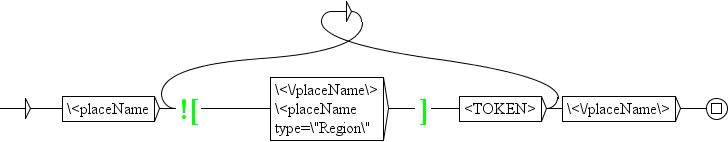
\includegraphics[width=15cm]{resources/img/placeNameHorsRegionStandoff.png}
  \caption{Graphe pour les balises \emph{placeName}, sauf celles de type \emph{Region}}
  \label{fig-placeNameHorsRegionStandoff}
\end{figure}

\noindent En passant une cascade avec le graphe de la figure~\ref{fig-placeNameHorsRegionStandoff},
on obtient un résultat avec une seule combinaison élément-type:
\begin{verbatim}
Voici les expressions trouvées :
     Liste pour l'élément "placeName" et l'attribut "City" 
          terme="Tours" 
          nombre=2 
     Fin de la liste pour cette paire.
Fin de la liste pour ce corpus
\end{verbatim}

\noindent Le fichier résultat est construit à partir d'un fichier modèle, dont on donne le nom en
ligne de commande avec l'option \verb$--standoff=<template file name>$.
Le fichier modèle est un fichier texte qui comprend au plus dix sections:

\begin{enumerate}
\item un texte introductif libre
\item une ligne contenant juste \verb$#LINE$: la partie entre \verb$#LINE$ et \verb$#REST$ servira
de modèle pour former dans le fichier résultat la partie sur un élément (ou sur une combinaison
élément-type)
\item un texte qui introduit un nom d'élément, noté \verb${TYPE}$, et éventuellement une valeur de
l'attribut \verb$type$, notée \verb${SUBTYPE}$. La partie optionnelle doit être délimitée entre
doubles chevrons: \verb$<<...>>$
\item une ligne \verb$#BLOCK$: la partie entre \verb$#BLOCK$ et \verb$#END$ servira de modèle
pour former dans le fichier résultat la partie sur une expression balisée
\item un texte introduisant une expression balisée, notée \verb${TERM}$
\item un texte introduisant le nombre d'occurrences de cette expression, noté \verb${COUNT}$
\item une ligne \verb$#END$
\item un texte signalant la fin de la partie sur un élément (ou sur une combinaison élément-type)
\item une ligne \verb$#REST$
\item un texte conclusif libre
\end{enumerate}

\noindent Voici le fichier modèle qui correspond à l'exemple ci-dessus:
\begin{verbatim}
Voici les expressions trouvées :
#LINE
     Liste pour l'élément "{TYPE}"<< et l'attribut "{SUBTYPE}">>
#BLOCK
          terme="{TERM}"
          nombre={COUNT}
#END
     Fin de la liste pour cette paire.
#REST
Fin de la liste pour ce corpus
\end{verbatim}

